\documentclass{article}

\usepackage{pgfplots}

\usepgfplotslibrary{fillbetween}

\begin{document}

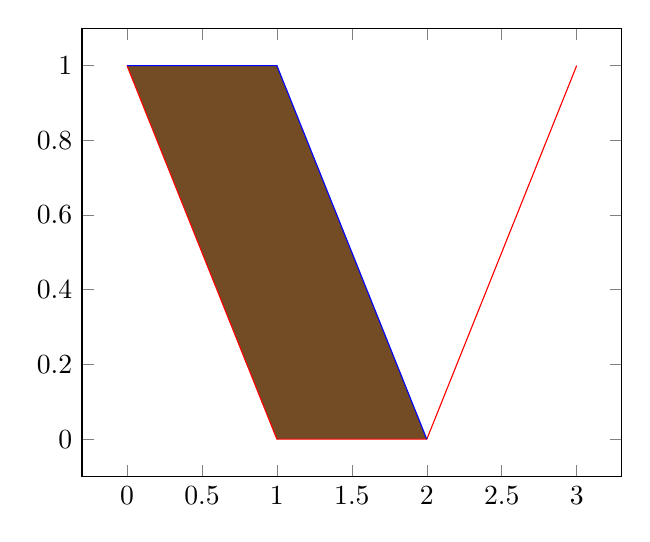
\begin{tikzpicture}
	\begin{axis}
	\addplot[red,name path=A, ] coordinates {
		(0,1) (1,0) (2,0) (3,1)
	};

	\addplot[blue,name path=B, ] coordinates {
		(0,1) (1,1) (2,0)
	};

	\addplot fill between[of = A and B,
	];

	\end{axis}
\end{tikzpicture}

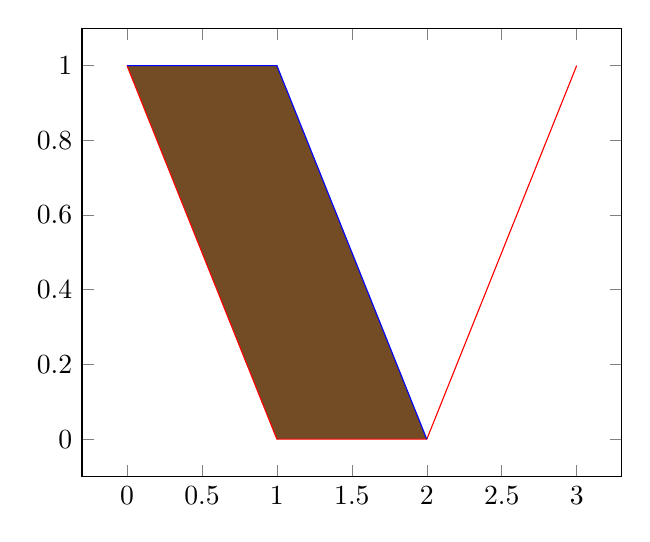
\begin{tikzpicture}
	\begin{axis}
	\addplot[red,name path=A, ] coordinates {
		(0,1) (1,0) (2,0) (3,1)
	};

	\addplot[blue,name path=B, ] coordinates {
		(0,1) (1,1) (2,0)
	};

	\addplot fill between[of = A and B,
		split,
	];

	\end{axis}
\end{tikzpicture}
\end{document}

